% =============================================================================
% Section 4: Results
% =============================================================================
\section{Results}
\label{sec:results}

We present results from the four forecast scenarios described in
Section~\ref{sec:scenarios}.  Readers encountering unfamiliar model
terminology (e.g., VBNC, force of infection, sweepstakes reproduction)
may wish to consult the Model Description
(Section~\ref{sec:model}) for mechanistic details.

Results focus on coast-wide population
trajectories (\S\ref{sec:trajectories}), regional recovery patterns
(\S\ref{sec:regional}), climate effects (\S\ref{sec:climate_effects}),
evolutionary dynamics (\S\ref{sec:evo_dynamics}), and the specific
question of how pathogen evolution shapes long-term outcomes
(\S\ref{sec:pathogen_evo}).  All numerical values are three-seed means
from the W154 production model.

% ---------------------------------------------------------------------------
\subsection{Population Trajectories}
\label{sec:trajectories}

\subsubsection{Coast-Wide Dynamics}

The coast-wide population trajectory under the baseline scenario (F01)
displays three distinct phases (Figure~\ref{fig:coastwide_population}).
The first phase is the initial catastrophic decline (2013--2015), during
which SSWD sweeps through virtually the entire range of
\textit{Pycnopodia helianthoides}, reducing coast-wide abundance by
more than 90\%.  This crash is driven by the combination of anomalously
warm SSTs during the 2013--2016 northeast Pacific marine heatwave and
the high initial susceptibility of host populations ($r_0 = 0.150$).

The second phase (2015--2025) is characterized by intermittent,
incomplete recovery attempts.  Recruitment pulses---transient surges in
juvenile abundance driven by seasonal cooling and residual reproductive
output---produce brief periods of apparent population growth, but these
gains are systematically erased during subsequent warm seasons when
pathogen activity resumes.  This ``two steps forward, one-and-a-half
steps back'' dynamic produces a sawtooth population trajectory with a
weak positive trend that fails to restore populations to pre-epizootic
levels.

The third phase (2025--2050) sees a gradual, secular decline as the
cumulative toll of recurring epizootics, progressive warming, and
pathogen adaptation erodes the demographic buffer.  By 2050, coast-wide
abundance under F01 stabilizes at approximately 238,687 individuals, or
5.4\% of the pre-disease peak of 4,447,241 (Table~\ref{tab:overall}).
The other three scenarios produce strikingly similar coast-wide outcomes:
F02 retains 5.9\% (261,632), F03 retains 5.1\% (224,638), and F04
retains 5.8\% (258,760).  The narrow range of these values
(5.1--5.9\%) belies dramatic regional redistribution, as detailed below.

\begin{table}[htbp]
\centering
\caption{Coast-wide population outcomes at 2050 across the four
forecast scenarios.  Values are three-seed means.}
\label{tab:overall}
\smallskip
\begin{tabular}{lrrr}
\toprule
\textbf{Scenario} & \textbf{Survivors} & \textbf{Initial} &
  \textbf{\% Surviving} \\
\midrule
F01 (SSP2-4.5, full evol.)       & 238,687 & 4,447,241 & 5.4 \\
F02 (SSP2-4.5, no evol.)         & 261,632 & 4,447,241 & 5.9 \\
F03 (SSP2-4.5, thermal only)     & 224,638 & 4,447,241 & 5.1 \\
F04 (SSP5-8.5, full evol.)       & 258,760 & 4,447,241 & 5.8 \\
\bottomrule
\end{tabular}
\end{table}

\subsubsection{Regional Divergence}

Beneath the superficially uniform coast-wide totals, regional
trajectories diverge markedly
(Figure~\ref{fig:regional_trajectories}).  Northern populations
(Alaska, British Columbia) display persistent seasonal cycling:
abundance builds during winter and spring when SSTs fall below the
pathogen's viable-but-non-culturable (VBNC) threshold, then declines
during summer and autumn as warming reactivates the pathogen.  This
oscillatory regime reflects the strong seasonality of high-latitude
SSTs and the proximity of ambient temperatures to the pathogen's
thermal activation boundary.

% --- Figure: Regional Trajectories ---
\begin{figure}[!htbp]
    \centering
    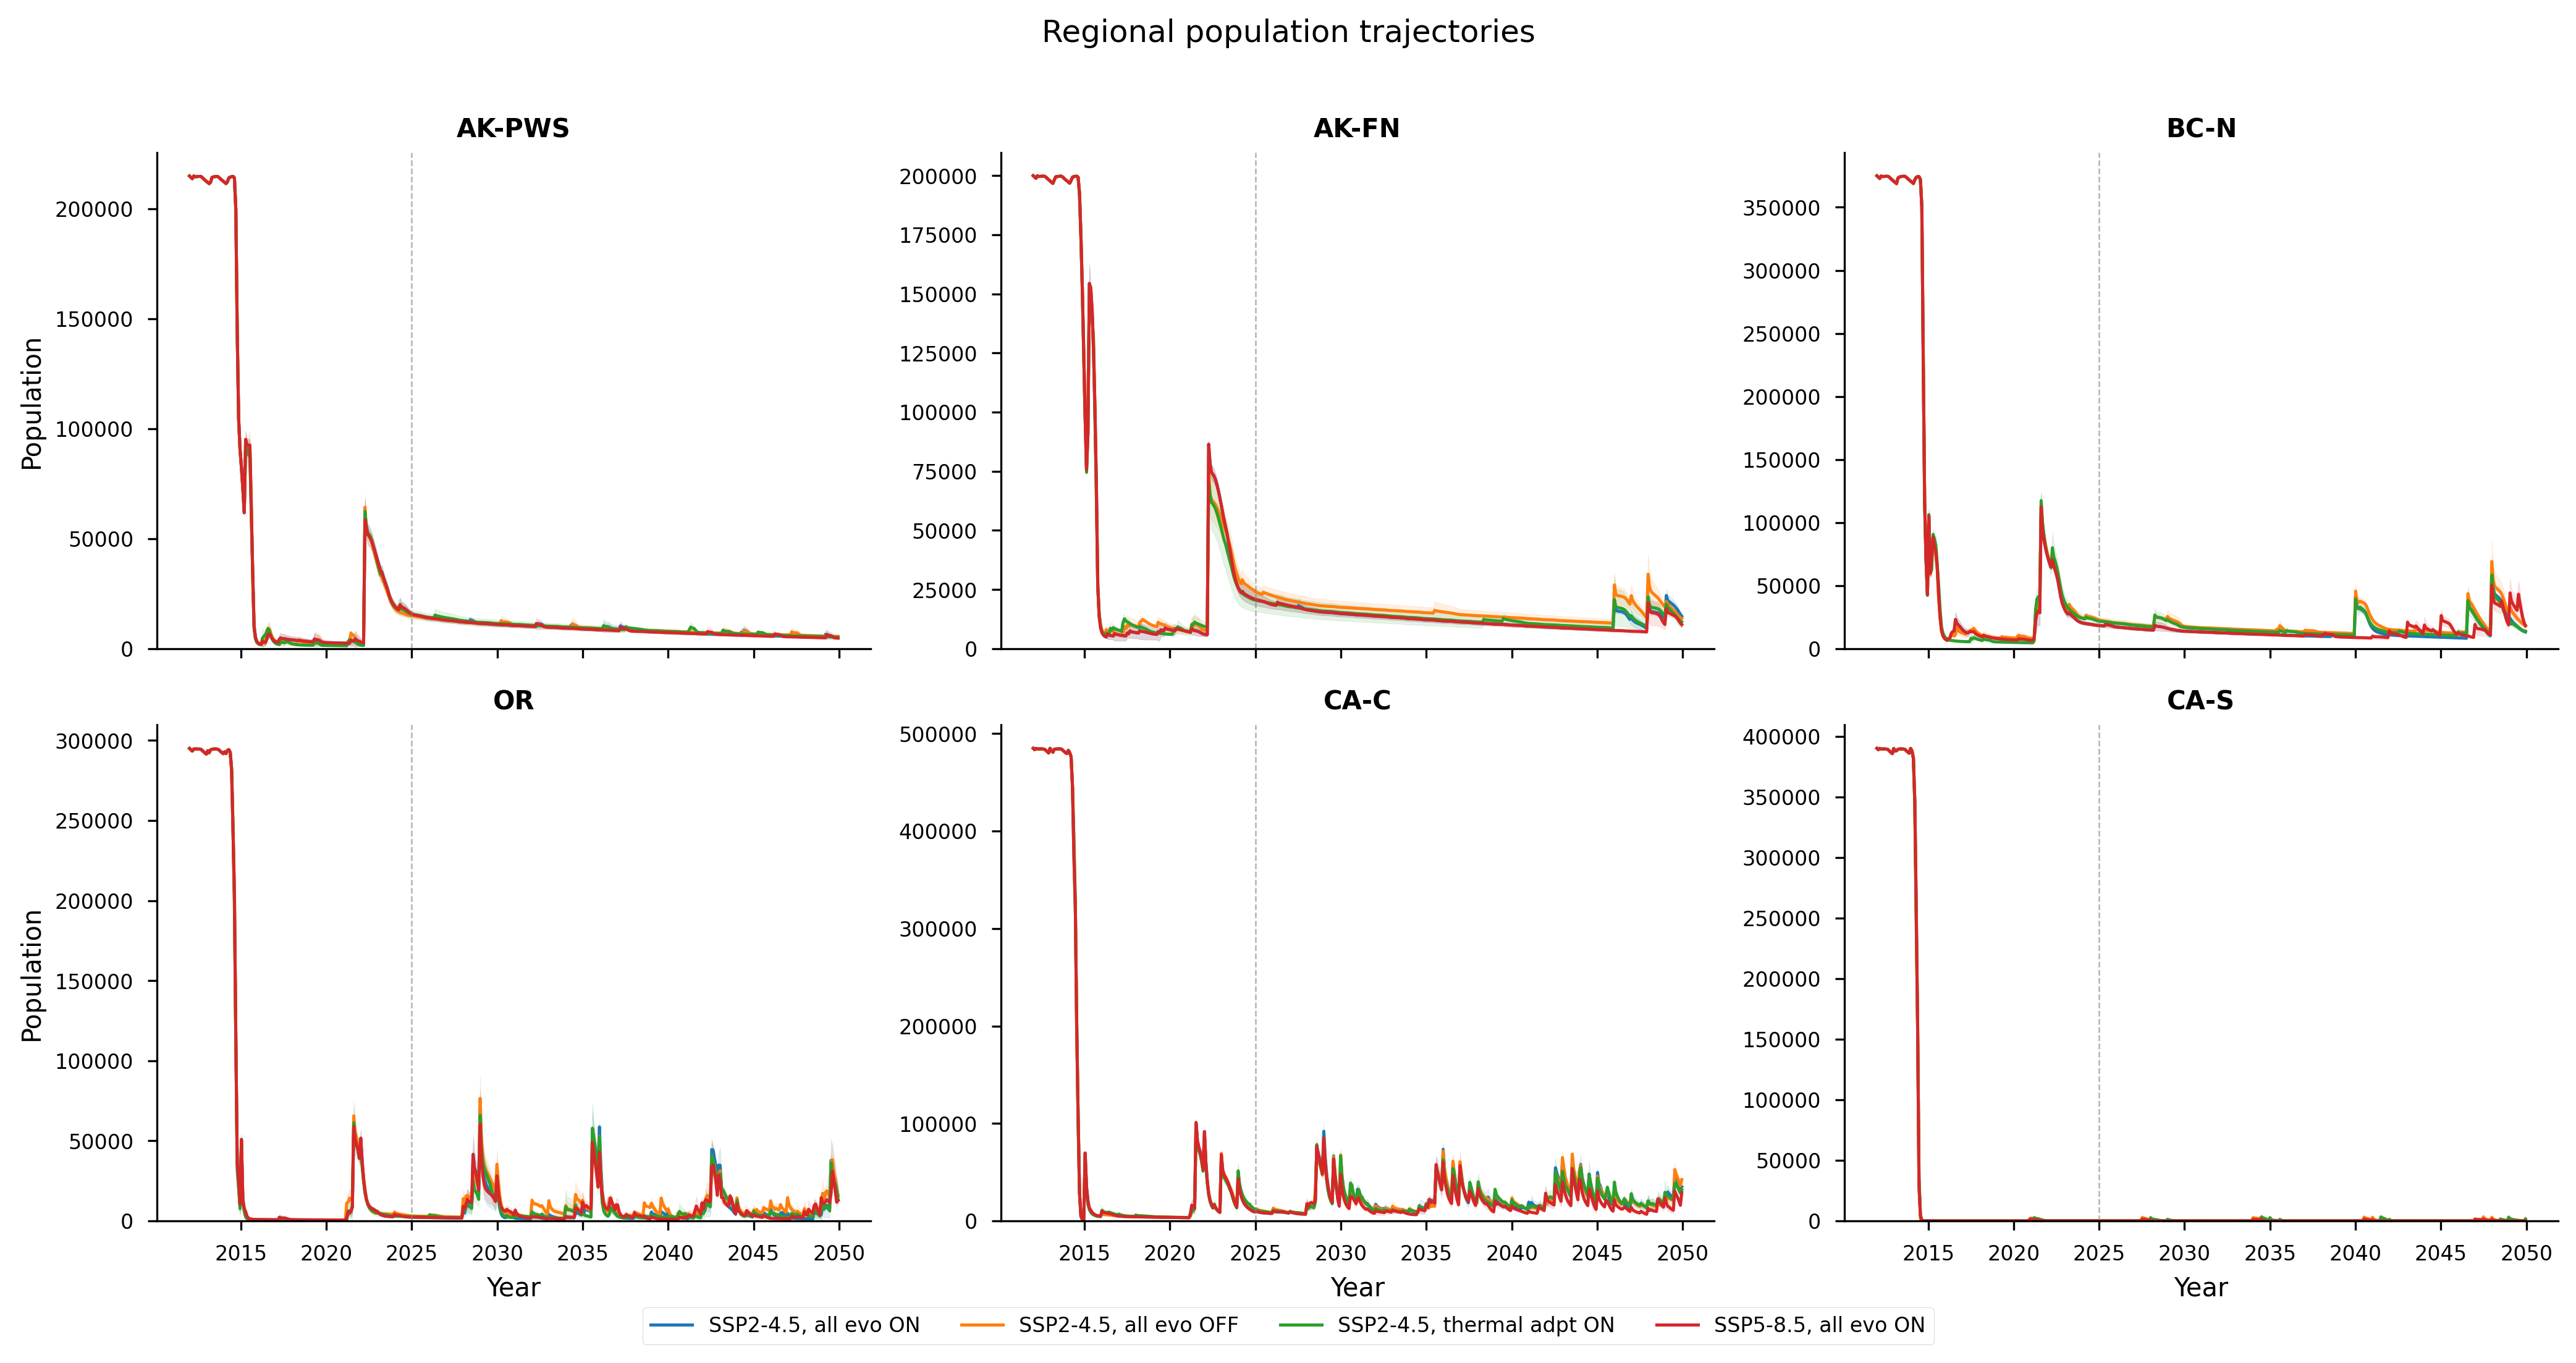
\includegraphics[width=\textwidth]{figures/fig_regional_trajectories.png}
    \caption{Population trajectories for six representative regions under all four scenarios. \textbf{Top row:} Alaska (AK-PWS, AK-FN) and British Columbia (BC-N), showing seasonal population cycling driven by winter pathogen dormancy and summer reactivation. \textbf{Bottom row:} Oregon (OR), central California (CA-C), and southern California (CA-S). Oregon sustains the highest long-term abundance; CA-S declines to extinction in all scenarios. Lines show three-seed means; shaded regions show $\pm$1 standard deviation.}
    \label{fig:regional_trajectories}
\end{figure}

In contrast, southern populations (California, Baja California) exhibit
monotonic decline with minimal seasonal modulation.  Year-round warm
SSTs in these regions maintain chronic pathogen activity, leaving
populations no seasonal refuge.  The result is a relentless erosion of
abundance that, in the most southerly regions, proceeds to functional
or absolute extinction (Section~\ref{sec:regional}).

% --- Figure: Regional Trajectories ---
\begin{figure}[!htbp]
    \centering
    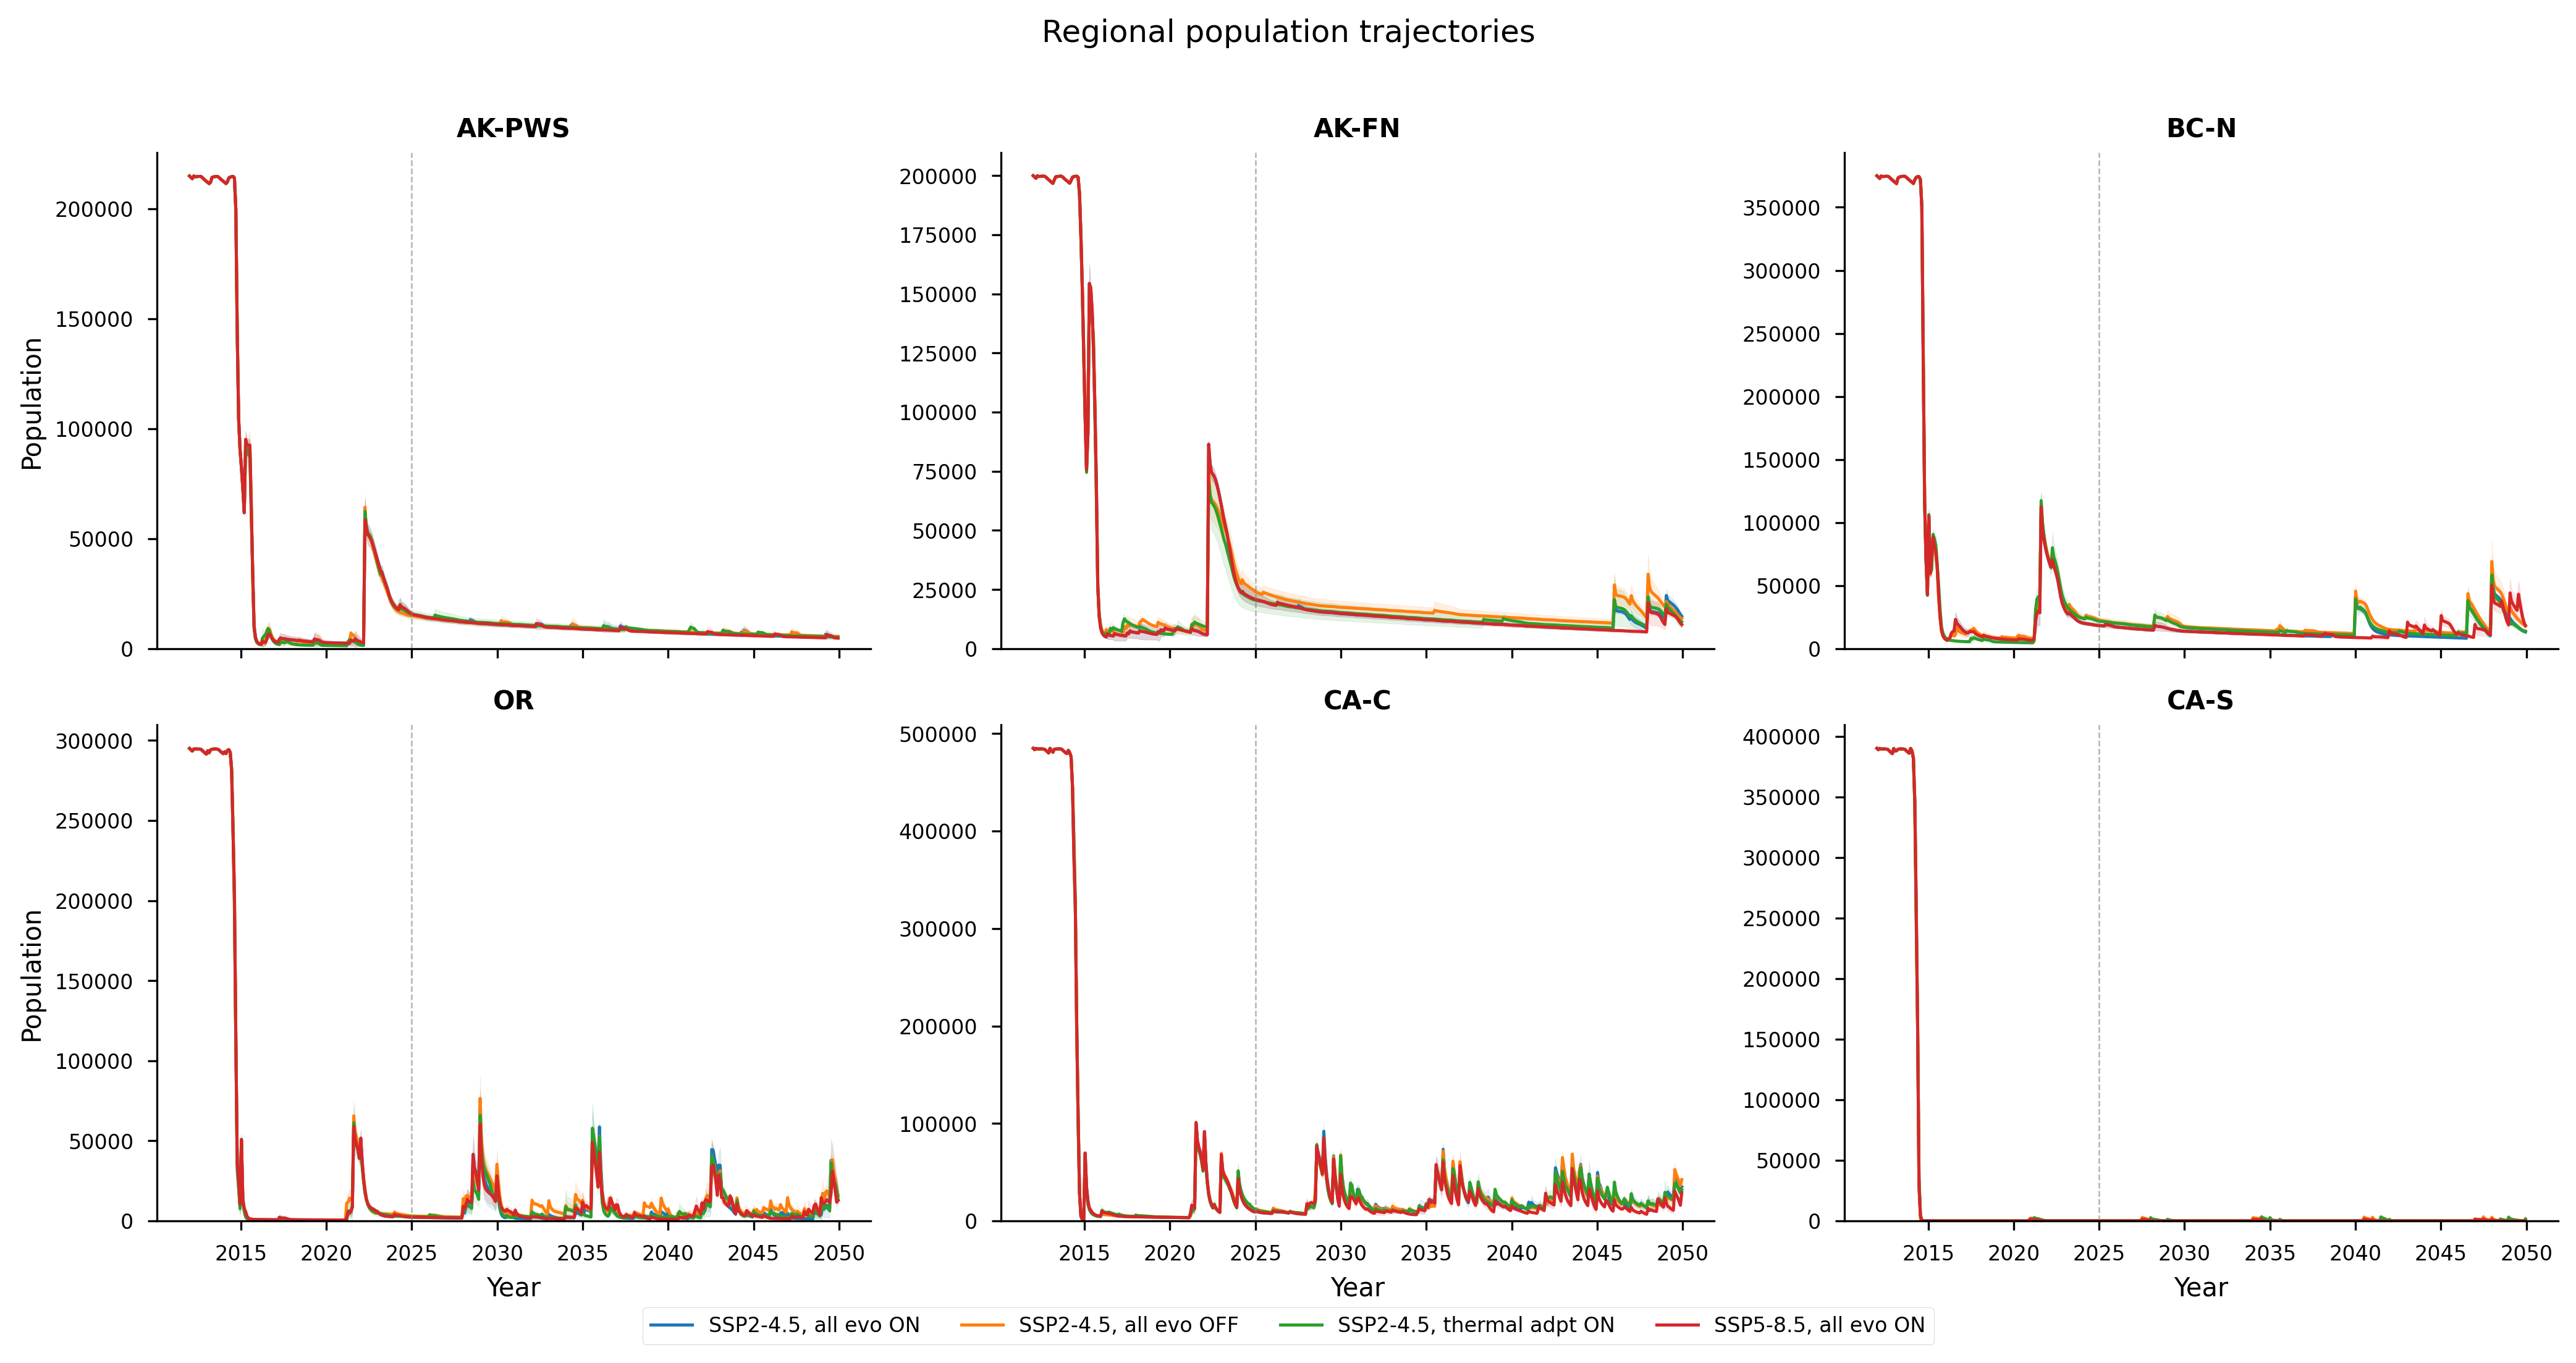
\includegraphics[width=\textwidth]{figures/fig_regional_trajectories.png}
    \caption{Population trajectories for six representative regions under all four scenarios. \textbf{Top row:} Alaska (AK-PWS, AK-FN) and British Columbia (BC-N), showing seasonal population cycling driven by winter pathogen dormancy and summer reactivation. \textbf{Bottom row:} Oregon (OR), central California (CA-C), and southern California (CA-S). Oregon shows episodic oasis dynamics with boom-bust cycles; CA-S declines to extinction in all scenarios. Lines show three-seed means; shaded regions show $\pm$1 standard deviation.}
    \label{fig:regional_trajectories}
\end{figure>

\subsubsection{The Recruitment Pulse Phenomenon}

A conspicuous feature of the simulated trajectories is the recurrence
of recruitment pulses---brief (2--6 month) surges in abundance that
interrupt the long-term decline.  These pulses arise when a sequence of
cooler-than-average months suppresses pathogen activity long enough for
surviving adults to reproduce and juveniles to recruit into the
population.  However, the pulses are inherently self-limiting: the
temporary increase in host density raises the effective contact rate,
and the subsequent return to warmer conditions triggers renewed
epizootic mortality that rapidly erases the demographic gain.

This dynamic is most pronounced in the mid-latitude transitional zone
(Washington, Oregon), where interannual SST variability is high and
the population teeters near the pathogen's thermal activation boundary.
In Alaska, pulses are smaller in amplitude but more regularly spaced,
tracking the predictable annual thermal cycle.  In southern California
and Baja, recruitment pulses are largely absent by the 2030s, as
chronic pathogen pressure suppresses reproduction below replacement
(Figure~\ref{fig:heatmap_population}).

% --- Figure: Population Heatmap ---
\begin{figure}[!htbp]
    \centering
    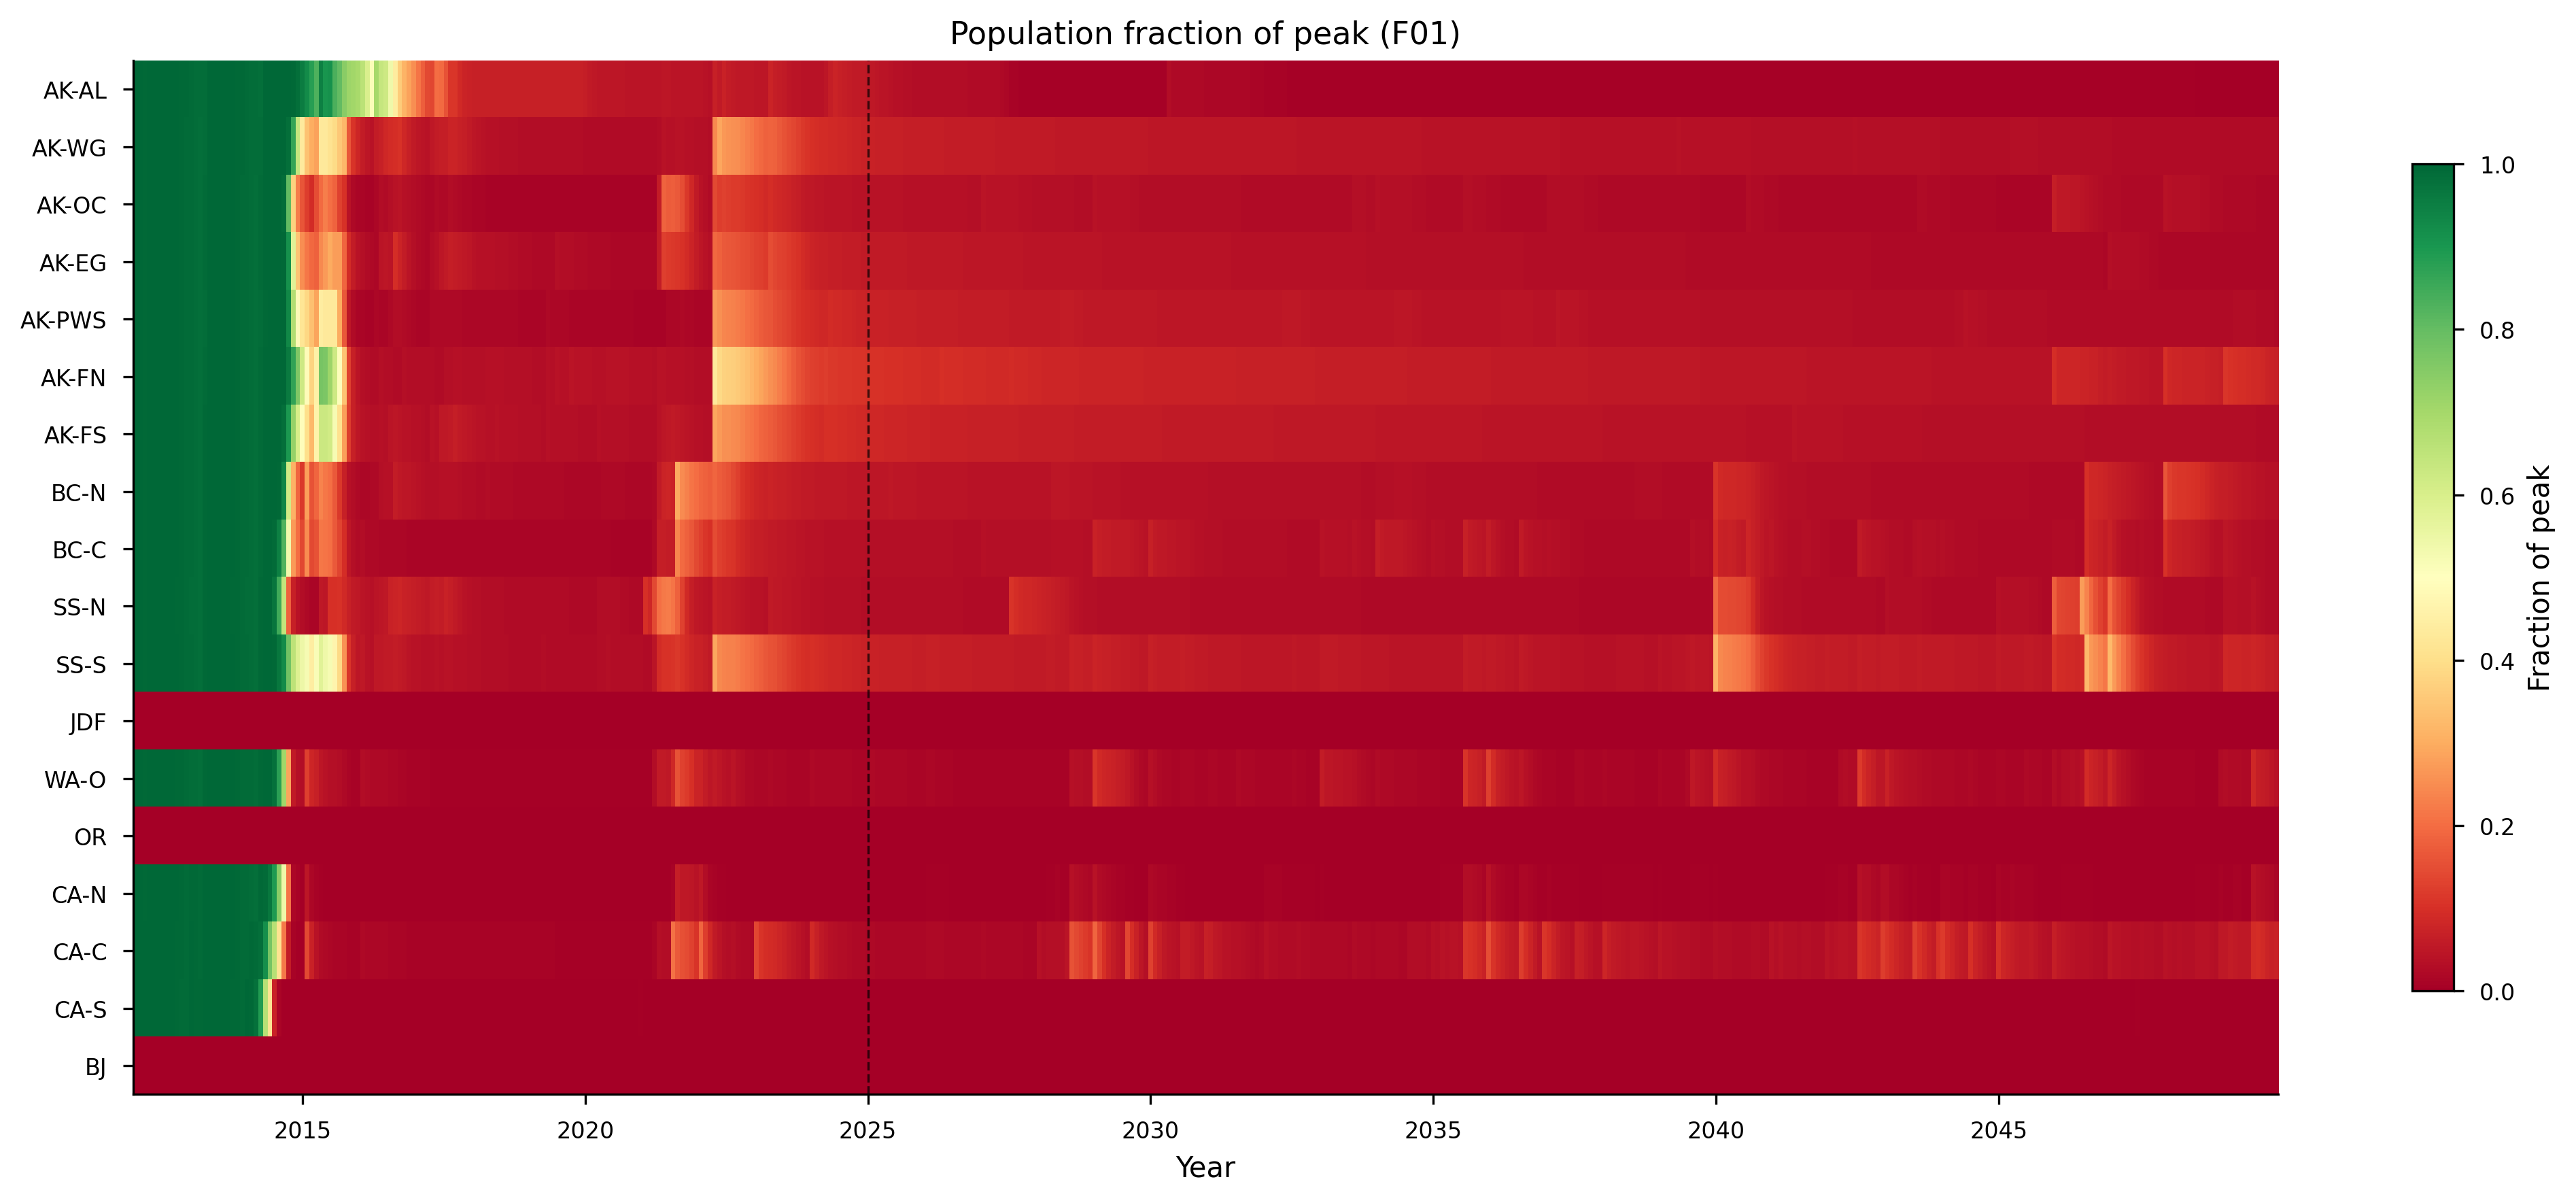
\includegraphics[width=\textwidth]{figures/fig_heatmap_population.png}
    \caption{Space--time heatmap of \textit{Pycnopodia} populations across the species' range under the baseline scenario (F01). Each row represents one of the 18 geographic regions (ordered south to north from bottom to top); the x-axis spans 2012--2050; color intensity indicates the fraction of carrying capacity occupied. The disease wavefront is visible as a dark band sweeping from south to north during 2013--2015. Post-crash, southern regions (BJ, CA-S) remain permanently dark (extinct), while a few northern and mid-latitude regions retain pale coloration (partial persistence). The 2025 observation-to-projection transition is marked.}
    \label{fig:heatmap_population}
\end{figure>

% ---------------------------------------------------------------------------
\subsection{Regional Recovery Patterns}
\label{sec:regional}

Table~\ref{tab:regional} presents the full matrix of regional recovery
percentages (surviving population as a fraction of initial abundance)
across all 18 model regions and four scenarios.

\begin{table}[htbp]
\centering
\caption{Regional recovery at 2050 (\% of initial population
surviving), grouped by geographic cluster.  Values are three-seed means.
Bold values indicate the highest recovery within each region across
scenarios. Note: Oregon's 17.6\% value represents an endpoint artifact; 
the 5-year average (2045--2050) is 5.4\% due to extreme boom-bust cycles.}
\label{tab:regional}
\smallskip
\small
\begin{tabular}{ll rrrr}
\toprule
\textbf{Cluster} & \textbf{Region} & \textbf{F01} & \textbf{F02} &
  \textbf{F03} & \textbf{F04} \\
\midrule
\multirow{7}{*}{\rotatebox[origin=c]{90}{\textbf{Alaska}}}
 & AK-AL  &  0.4 & \textbf{4.1} &  0.7 &  0.4 \\
 & AK-WG  &  2.5 & \textbf{4.5} &  3.0 &  2.4 \\
 & AK-OC  &  1.8 &  3.1          &  1.5 & \textbf{6.0} \\
 & AK-EG  &  1.7 & \textbf{2.4} &  2.0 &  1.6 \\
 & AK-PWS &  2.4 & \textbf{2.6} &  2.5 &  2.2 \\
 & AK-FN  &  6.8 &  6.4          &  5.7 & \textbf{9.9} \\
 & AK-FS  &  2.7 &  3.6          &  2.9 & \textbf{10.3} \\
\midrule
\multirow{4}{*}{\rotatebox[origin=c]{90}{\textbf{BC/SS}}}
 & BC-N   &  3.6 &  4.9          &  3.7 & \textbf{11.3} \\
 & BC-C   &  3.3 & \textbf{7.5} &  4.1 &  6.4 \\
 & SS-N   &  2.4 & \textbf{3.6} &  2.6 &  3.1 \\
 & SS-S   &  6.5 & \textbf{8.8} &  7.7 &  7.6 \\
\midrule
\multirow{3}{*}{\rotatebox[origin=c]{90}{\textbf{PNW}}}
 & JDF    &  5.4 & \textbf{6.5} &  5.9 &  5.3 \\
 & WA-O   & \textbf{8.8} &  5.1 &  4.2 &  6.0 \\
 & OR     & \textbf{17.6} & 12.8 & 15.3 & 10.4 \\
\midrule
\multirow{4}{*}{\rotatebox[origin=c]{90}{\textbf{CA/BJ}}}
 & CA-N   &  5.0 & \textbf{5.9} &  2.9 &  4.3 \\
 & CA-C   & \textbf{11.9} & 11.9 & 11.5 &  7.6 \\
 & CA-S   &  0.0 &  0.1          & \textbf{0.4} &  0.0 \\
 & BJ     &  0.0 &  0.0          &  0.0 &  0.0 \\
\bottomrule
\end{tabular}
\end{table}

\subsubsection{Alaska}

Alaskan populations uniformly show poor recovery across all scenarios,
with most regions retaining fewer than 3\% of initial abundance under
the baseline (F01).  The exception is AK-FN (Funter Bay--northern
Southeast Alaska), which achieves 6.8\% under F01 and reaches 9.9\%
under the high-warming scenario F04.  The consistently low values
throughout western and south-central Alaska reflect the combination of
cold winters that limit the reproductive season and summers that,
despite being cool by lower-latitude standards, are now warm enough to
sustain episodic pathogen outbreaks.

Notably, several Alaskan regions show their strongest recovery under
F04 (SSP5-8.5), particularly AK-FS (+7.6 percentage points relative to
F01) and AK-OC (+4.2 points).  This counterintuitive result---warming
\textit{helping} northern populations---is discussed in
Section~\ref{sec:climate_effects}.

\subsubsection{British Columbia and the Salish Sea}

British Columbia and the Salish Sea region display moderate recovery
potential (3--9\%) with substantial sensitivity to both climate and
evolutionary scenarios.  BC-N (northern British Columbia) is among the
most climate-responsive regions in the entire domain, increasing from
3.6\% under F01 to 11.3\% under F04---a gain of 7.7 percentage
points that makes it the single largest beneficiary of high-end warming
(Figure~\ref{fig:regional_recovery_bars}).  BC-C (central British
Columbia) is instead most sensitive to pathogen evolution, jumping from
3.3\% (F01) to 7.5\% (F02, evolution off), a gain of 4.2 points.

The Salish Sea subregions (SS-N, SS-S) exhibit intermediate recovery
and moderate scenario sensitivity.  SS-S consistently outperforms SS-N,
likely reflecting the greater habitat complexity and cooler deep-water
refugia of the southern basins.

\subsubsection{Pacific Northwest: Oregon's Episodic Dynamics}

The Pacific Northwest cluster reveals the most striking regional
pattern in the entire forecast ensemble.  Oregon (OR) appears to be 
the recovery leader in 2050 endpoint snapshots (17.6\%), but this 
reflects boom-bust episodic dynamics rather than sustained recovery. 
Oregon's 5-year average (2045--2050) is 5.4\% with 121\% coefficient 
of variation, indicating extreme volatility. Alaska's Fairweather-North 
region shows more reliable persistence (6.8\% snapshot, 9.4\% 5-year 
average). Oregon's episodic advantage derives from oasis sites that 
periodically boom due to strong upwelling, thermal variability, and 
sweepstakes reproductive success, but these gains are repeatedly erased 
by subsequent pathogen activity.

However, Oregon's episodic dynamics are also highly vulnerable to both 
warming and evolutionary change.  Under F04 (high warming), Oregon's 
endpoint snapshot drops to 10.4\%---a loss of 7.2 percentage points 
affecting both snapshots and underlying averages, the largest negative
climate effect of any region.  Under F02 (no evolution), Oregon's 
endpoint declines to 12.8\%, losing 4.8 points despite the coast-wide 
benefit of freezing pathogen evolution.  These paradoxical vulnerabilities 
reflect the fragility of Oregon's oasis-driven boom-bust cycles and are
analyzed in Sections~\ref{sec:climate_effects} and \ref{sec:pathogen_evo}.

Outer Washington (WA-O) follows a distinctive pattern, achieving its
highest recovery (8.8\%) under F01 but declining under all alternative
scenarios---including F02, where disabling pathogen evolution actually
reduces its recovery by 3.7 percentage points.

\subsubsection{California and Baja California: Southern Collapse}

Southern California (CA-S) and Baja California (BJ) are functionally
extinct across all scenarios.  CA-S retains at most 0.4\% of its
initial population (under F03), while BJ achieves 0.0\% in every
scenario.  These results indicate that even under moderate warming with
favorable evolutionary assumptions, the southern range limit of
\textit{P.~helianthoides} has contracted northward past approximately
33\textdegree N and is unlikely to recover within the forecast horizon.

Central California (CA-C) presents a more nuanced picture: it maintains
robust recovery (11.9\%) under both F01 and F02 but declines
substantially (to 7.6\%) under high warming (F04).  Northern California
(CA-N) is intermediate, with moderate recovery (5.0--5.9\%) under
SSP2-4.5 scenarios but reduced persistence (4.3\%) under SSP5-8.5.

The extinction of southern populations represents the loss of a
significant fraction of the species' historical genetic diversity and
raises conservation concerns that extend beyond simple abundance
metrics (Section~\ref{sec:evo_dynamics}).

% ---------------------------------------------------------------------------
\subsection{Climate Effects}
\label{sec:climate_effects}

The contrast between F01 (SSP2-4.5) and F04 (SSP5-8.5), both with
full evolutionary dynamics, isolates the effect of enhanced ocean
warming on population outcomes.  Coast-wide, the net effect is
remarkably small: F04 retains 5.8\% of the initial population versus
5.4\% under F01, a difference of only +0.4 percentage points.  This
near-zero aggregate effect, however, masks a dramatic latitudinal
redistribution of surviving populations
(Figure~\ref{fig:climate_effect}).

\subsubsection{Northern Beneficiaries}

The largest positive climate effects are concentrated in a band from
southern Alaska through northern British Columbia
(Figure~\ref{fig:recovery_vs_latitude}):

% --- Figure: Recovery vs Latitude ---
\begin{figure}[!htbp]
    \centering
    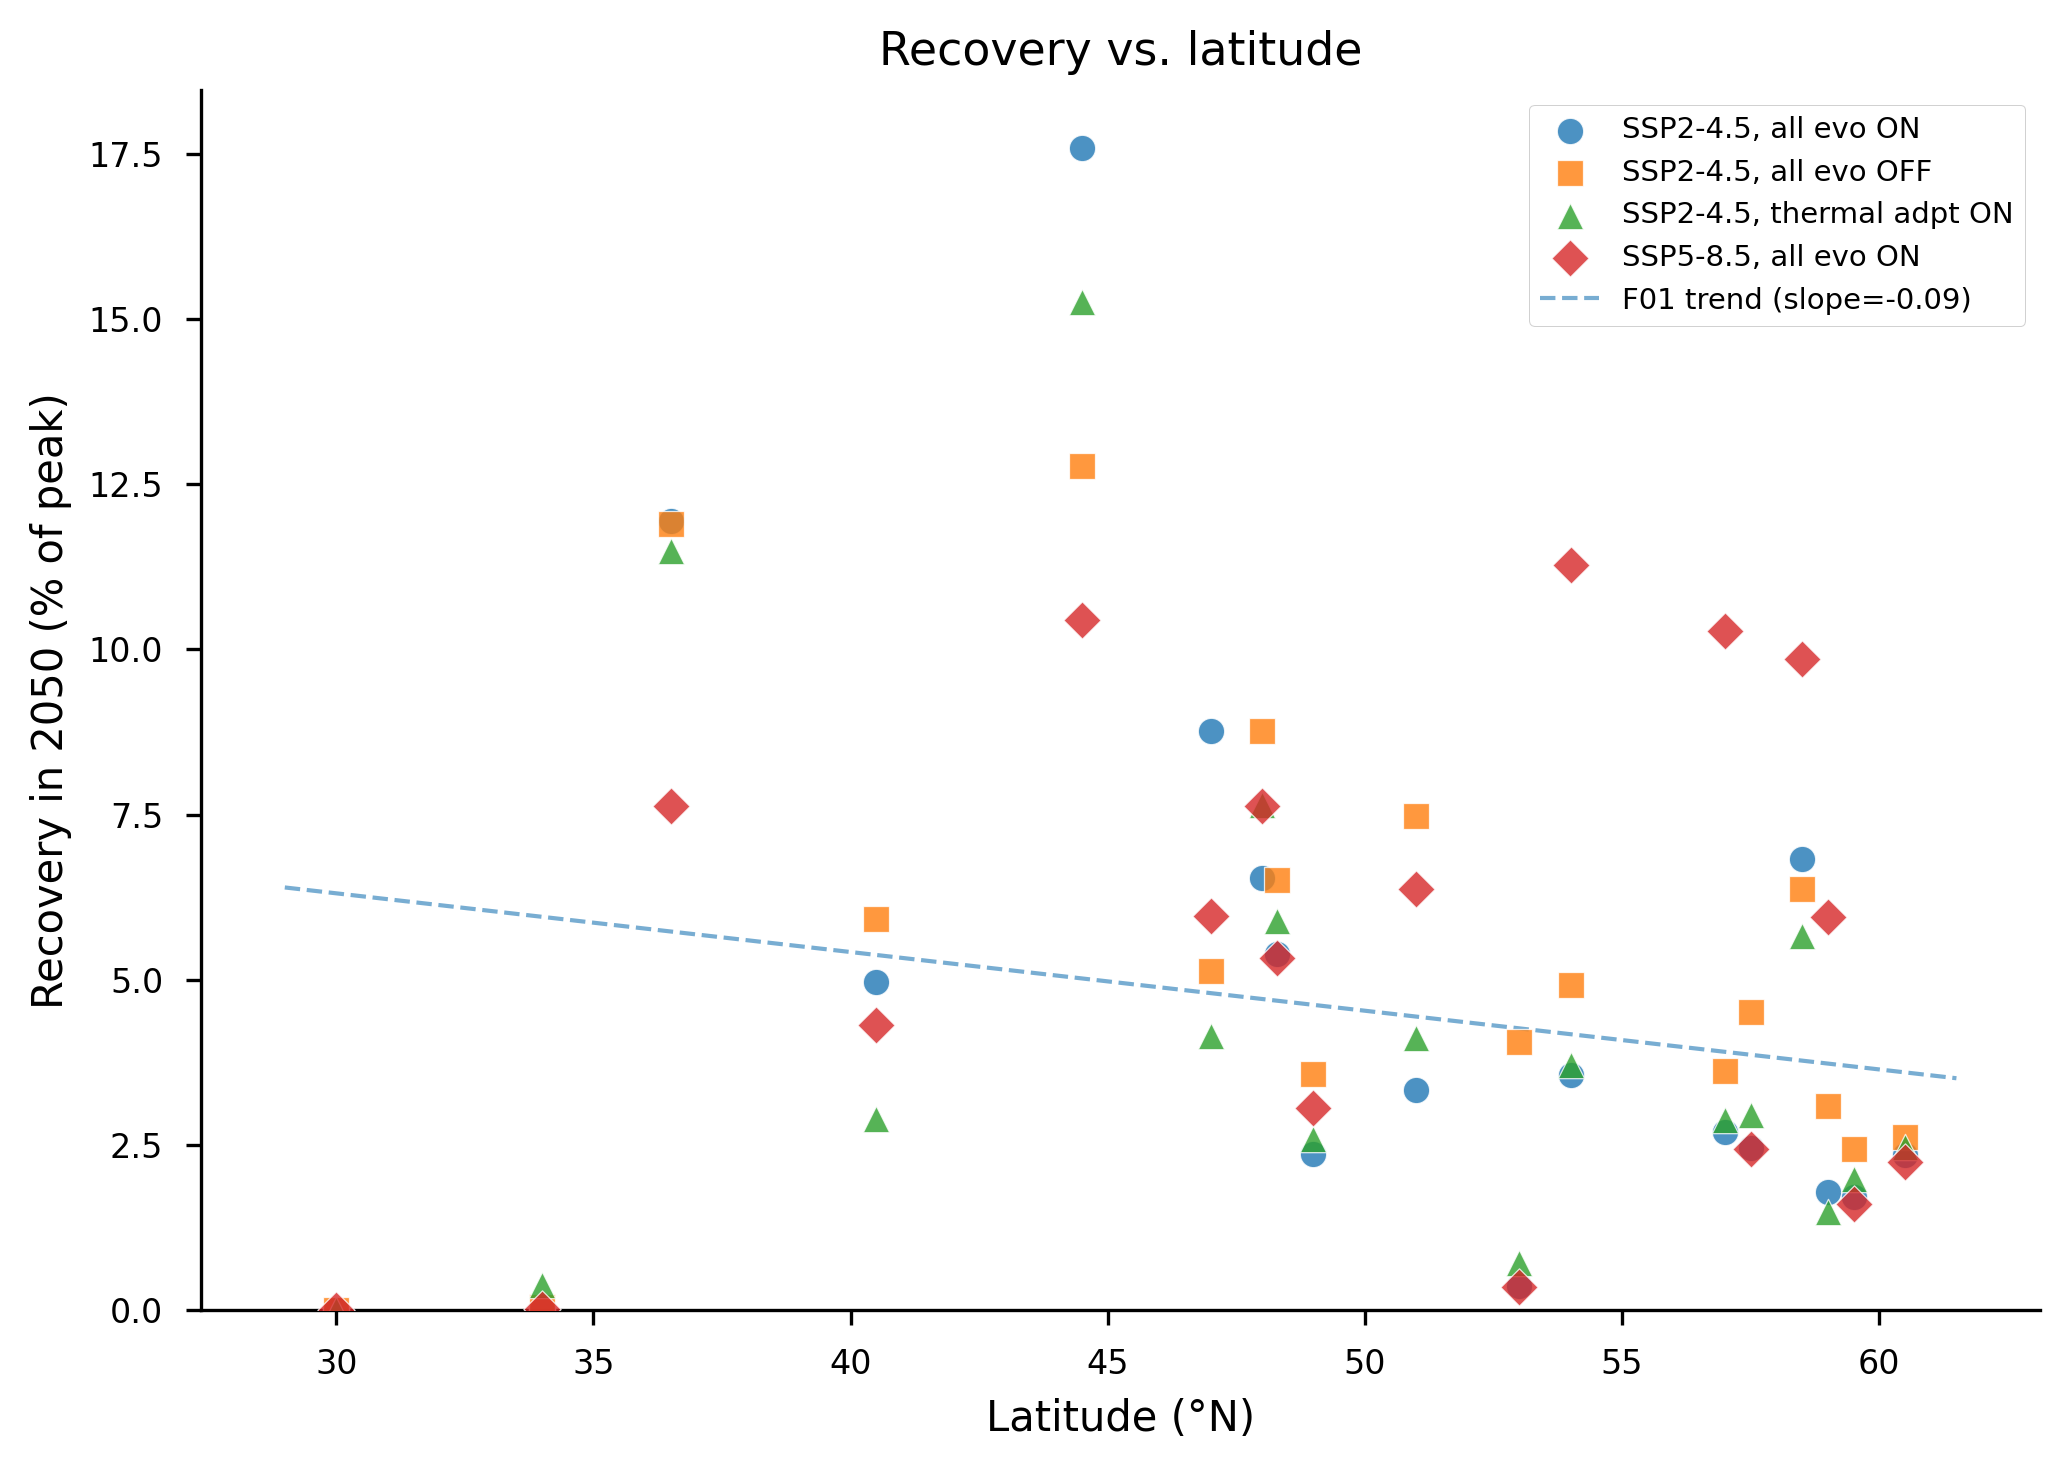
\includegraphics[width=0.75\textwidth]{figures/fig_recovery_vs_latitude.png}
    \caption{Recovery fraction vs.\ latitude for all 18 regions across four scenarios. Each point represents a region's three-seed mean recovery percentage at 2050. Under baseline conditions (F01, blue), Oregon ($\sim$45\textdegree N) shows a 2050 endpoint artifact of 17.6\% (5-year average: 5.4\% with high variability), while Alaska's Fairweather-North provides more reliable recovery. Under high warming (F04, red), the high-latitude tail lifts substantially while the mid-latitude peak flattens, reflecting the northward shift in favorable conditions. The relationship between latitude and recovery is nonlinear and non-monotonic, driven by the interplay of temperature-dependent pathogen activity, host reproductive season length, and site-specific hydrodynamic flushing.}
    \label{fig:recovery_vs_latitude}
\end{figure>

\begin{itemize}
  \item BC-N: $+$7.7 percentage points (3.6\% $\rightarrow$ 11.3\%)
  \item AK-FS: $+$7.6 points (2.7\% $\rightarrow$ 10.3\%)
  \item AK-OC: $+$4.2 points (1.8\% $\rightarrow$ 6.0\%)
  \item AK-FN: $+$3.1 points (6.8\% $\rightarrow$ 9.9\%)
  \item BC-C: $+$3.1 points (3.3\% $\rightarrow$ 6.4\%)
\end{itemize}

\noindent
The mechanism underlying this northern benefit operates through two
complementary pathways.  First, warming extends the effective growing
season for \textit{P.~helianthoides} at high latitudes, where
cold-limited reproduction constrains population growth rates more
severely than disease-induced mortality during most of the year.
Second, although warming also extends the pathogen's active season,
the absolute SSTs in these regions remain near the lower boundary of
the pathogen's thermal niche even under SSP5-8.5, limiting the
intensity and duration of summer epizootics.  The net balance thus
favors the host: more reproduction in spring and autumn, with only
modestly increased disease pressure in summer.

\subsubsection{Southern Losers}

South of approximately 48\textdegree N, warming uniformly depresses
recovery:

\begin{itemize}
  \item OR: $-$7.2 percentage points (17.6\% $\rightarrow$ 10.4\%)
  \item CA-C: $-$4.3 points (11.9\% $\rightarrow$ 7.6\%)
  \item WA-O: $-$2.8 points (8.8\% $\rightarrow$ 6.0\%)
  \item CA-N: $-$0.7 points (5.0\% $\rightarrow$ 4.3\%)
\end{itemize}

\noindent
In these regions, baseline SSTs are already warm enough to sustain
prolonged pathogen activity.  Additional warming expands the window of
active transmission into what were previously marginal shoulder
seasons, increasing the cumulative annual disease burden.
Simultaneously, these populations are already near the upper thermal
tolerance for reproduction, so warming provides little compensatory
demographic benefit.  Oregon suffers the steepest absolute decline
because it has the most to lose: its high baseline recovery rate
amplifies the proportional impact of extended pathogen activity seasons.

\subsubsection{The Breakeven Latitude}

The transition from net climate benefit (north) to net climate cost
(south) occurs at approximately 48\textdegree N---roughly the latitude
of the Juan de Fuca Strait and the boundary between the
upwelling-dominated California Current system and the downwelling
regime of the northern shelf.  This breakeven latitude is not merely a
statistical artifact but reflects a genuine biophysical boundary: north
of 48\textdegree N, winter SSTs are sufficiently cold that the pathogen
enters prolonged VBNC dormancy, and warming's primary effect is to
accelerate host population growth during the expanded ice-free season.
South of this boundary, the pathogen's dormancy period is already short
or absent, and warming's primary effect is to intensify chronic disease
pressure.

The existence of this breakeven latitude has important conservation
implications.  Under high-end warming, the center of abundance for
\textit{P.~helianthoides} shifts northward by several degrees of
latitude, with northern British Columbia and southeastern Alaska
emerging as the primary refugia.  This geographic shift could alter the
species' ecological role along the coast, as regions that currently
benefit from sunflower star predation on sea urchins (notably the
California kelp forests) would lose this keystone function while
regions with less acute urchin overgrazing pressure gain it.

% ---------------------------------------------------------------------------
\subsection{Evolutionary Dynamics}
\label{sec:evo_dynamics}

The coupled eco-evolutionary framework tracks the temporal evolution of
both host resistance and pathogen traits at each of the 896 model
sites.  Under the baseline scenario (F01), these traits exhibit
striking spatial gradients and temporal dynamics that illuminate the
interplay between selection, drift, and demographic constraint.

\subsubsection{Host Resistance}

Mean host resistance ($\bar{r}$) increases from the uniform initial
value of 0.150 toward higher values in all surviving populations, but
the rate and ultimate level of resistance evolution vary enormously
across the latitudinal range
(Figure~\ref{fig:resistance_evolution}):

\begin{itemize}
  \item \textbf{Alaska (moderate selection, slow response):}
    AK-PWS: $0.150 \rightarrow 0.253$;
    AK-FN: $0.150 \rightarrow 0.230$.
    Disease pressure is seasonal and moderate, producing
    consistent but gentle directional selection.
  \item \textbf{British Columbia (intermediate):}
    BC-N: $0.150 \rightarrow 0.240$.
    Stronger summer epizootics drive faster allele frequency
    change than in Alaska, but demographic stability maintains
    sufficient population sizes for effective selection.
  \item \textbf{Oregon and California (intense selection, rapid
    response):}
    OR: $0.150 \rightarrow 0.378$;
    CA-C: $0.150 \rightarrow 0.425$.
    Year-round pathogen activity imposes sustained, intense
    selection for resistance.  CA-C achieves the highest
    resistance of any surviving population, with mean $\bar{r}$
    reaching 0.43 by 2050.
  \item \textbf{Southern California (extinction):}
    CA-S: $0.150 \rightarrow 0.115$ (approximately 52 survivors).
    Mean resistance actually \textit{declines} below the starting
    value, because the population is so small (${\sim}$50 individuals)
    that genetic drift overwhelms directional selection.
\end{itemize}

\noindent
A critical observation is that even the highest evolved resistance
level ($\bar{r} = 0.425$ in CA-C) provides only partial protection:
at this resistance level, 58\% of the force of infection still
penetrates host defenses.  In the context of the model's multiplicative
disease framework, this means that CA-C populations in 2050 still
experience more than half the per-capita disease mortality of a
completely na\"ive population.  Resistance evolution slows the decline
but does not arrest it.

\subsubsection{The Cruel Paradox of Evolutionary Capacity}

The populations under the most intense selection for resistance are
precisely those with the least capacity to respond.  In southern
populations, chronic pathogen pressure drives rapid allele frequency
change but simultaneously erodes population size, reducing the
effective population size ($N_e$) and hence the efficiency of
selection.  As $N_e$ declines, genetic drift increasingly overwhelms
directional selection, and the additive genetic variance available for
further adaptation collapses
(Figure~\ref{fig:genetic_diversity}).

This evolutionary trap is starkest in CA-S, where the population
declines to approximately 52 individuals by 2050 despite experiencing
intense selection pressure.  Remarkably, the mean resistance of these
survivors ($\bar{r} = 0.115$) is actually \textit{lower} than the
starting value (0.150)---evidence that in such a tiny population,
genetic drift has overwhelmed directional selection.  The few surviving
individuals are not the ``most resistant''; they are simply the ones
that happened to survive through stochastic chance.  Allee effects
and demographic stochasticity now dominate their fate far more than
any genetic advantage.

The paradox generalizes across the southern range: the populations that
``need'' evolutionary rescue the most are those least likely to achieve
it, because the disease that creates the selection pressure also
destroys the demographic base required for effective evolutionary
response.  This result echoes theoretical predictions from
evolutionary rescue theory \citep{gomulkiewicz1995, bell2008} and
provides a concrete, spatially explicit demonstration of its
consequences for a real species undergoing an ongoing epizootic.

% --- Figure: Genetic Diversity ---
\begin{figure}[!htbp]
    \centering
    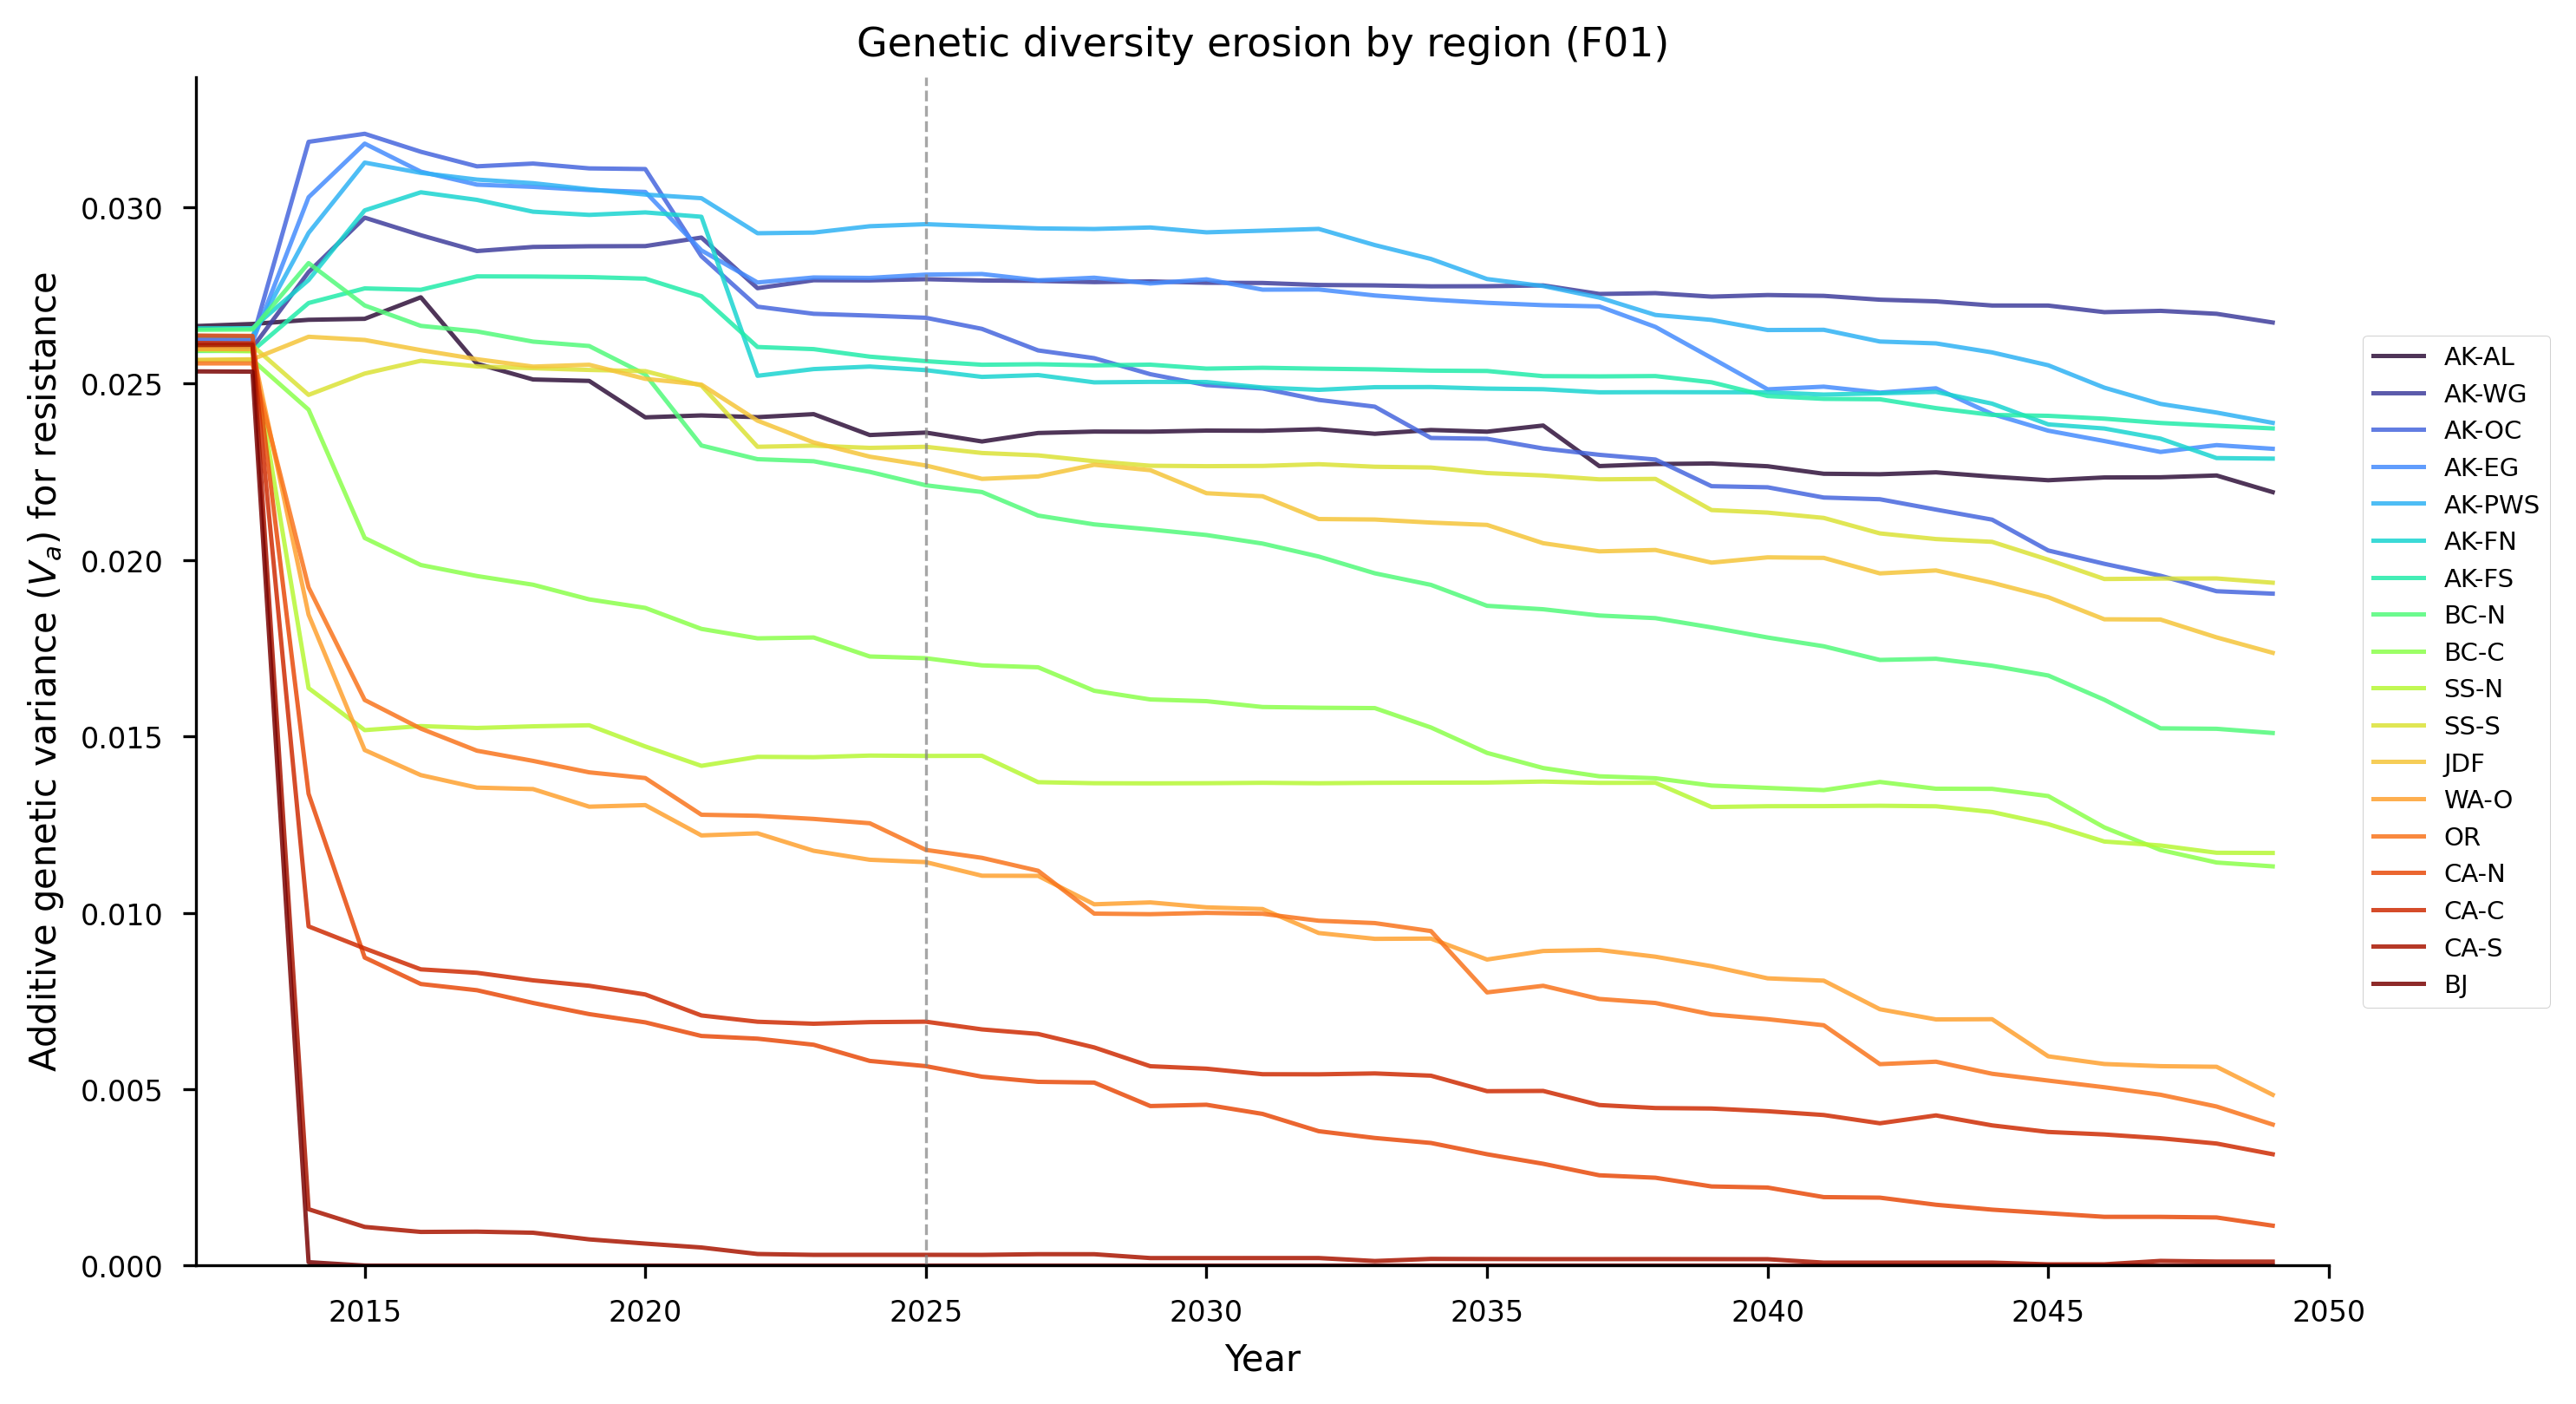
\includegraphics[width=0.75\textwidth]{figures/fig_genetic_diversity.png}
    \caption{Additive genetic variance ($V_A$) for the resistance trait across six regions under the baseline scenario (F01). $V_A$ measures the raw material available for future evolutionary adaptation. Southern populations (CA-C, CA-S) lose genetic diversity rapidly as intense disease selection eliminates most genotypes. By 2050, CA-C retains only a fraction of its initial $V_A$---the population has evolved substantially but is running out of ``evolutionary fuel.' Northern populations (AK-PWS, AK-FN) maintain higher $V_A$ because weaker selection preserves more genotypic diversity. This creates a cruel paradox: the populations that most need to evolve have the least remaining capacity to do so.}
    \label{fig:genetic_diversity}
\end{figure}

\subsubsection{Pathogen Thermal Adaptation}

The pathogen's VBNC threshold temperature ($T_\mathrm{vbnc}$)---the
SST below which the pathogen enters dormancy---evolves toward lower
values in cold-water regions as strains with broader thermal niches
gain a fitness advantage through extended transmission seasons.  By
2050 under F01, $T_\mathrm{vbnc}$ has declined to its implemented
lower bound of 9.00\textdegree C throughout Alaska (AK-PWS:
9.00\textdegree C; AK-FN: 9.00\textdegree C), indicating that
selection has driven the trait to the edge of the modeled parameter
space within 38 years (Figure~\ref{fig:pathogen_traits}).

% --- Figure: Pathogen Traits ---
\begin{figure}[!htbp]
    \centering
    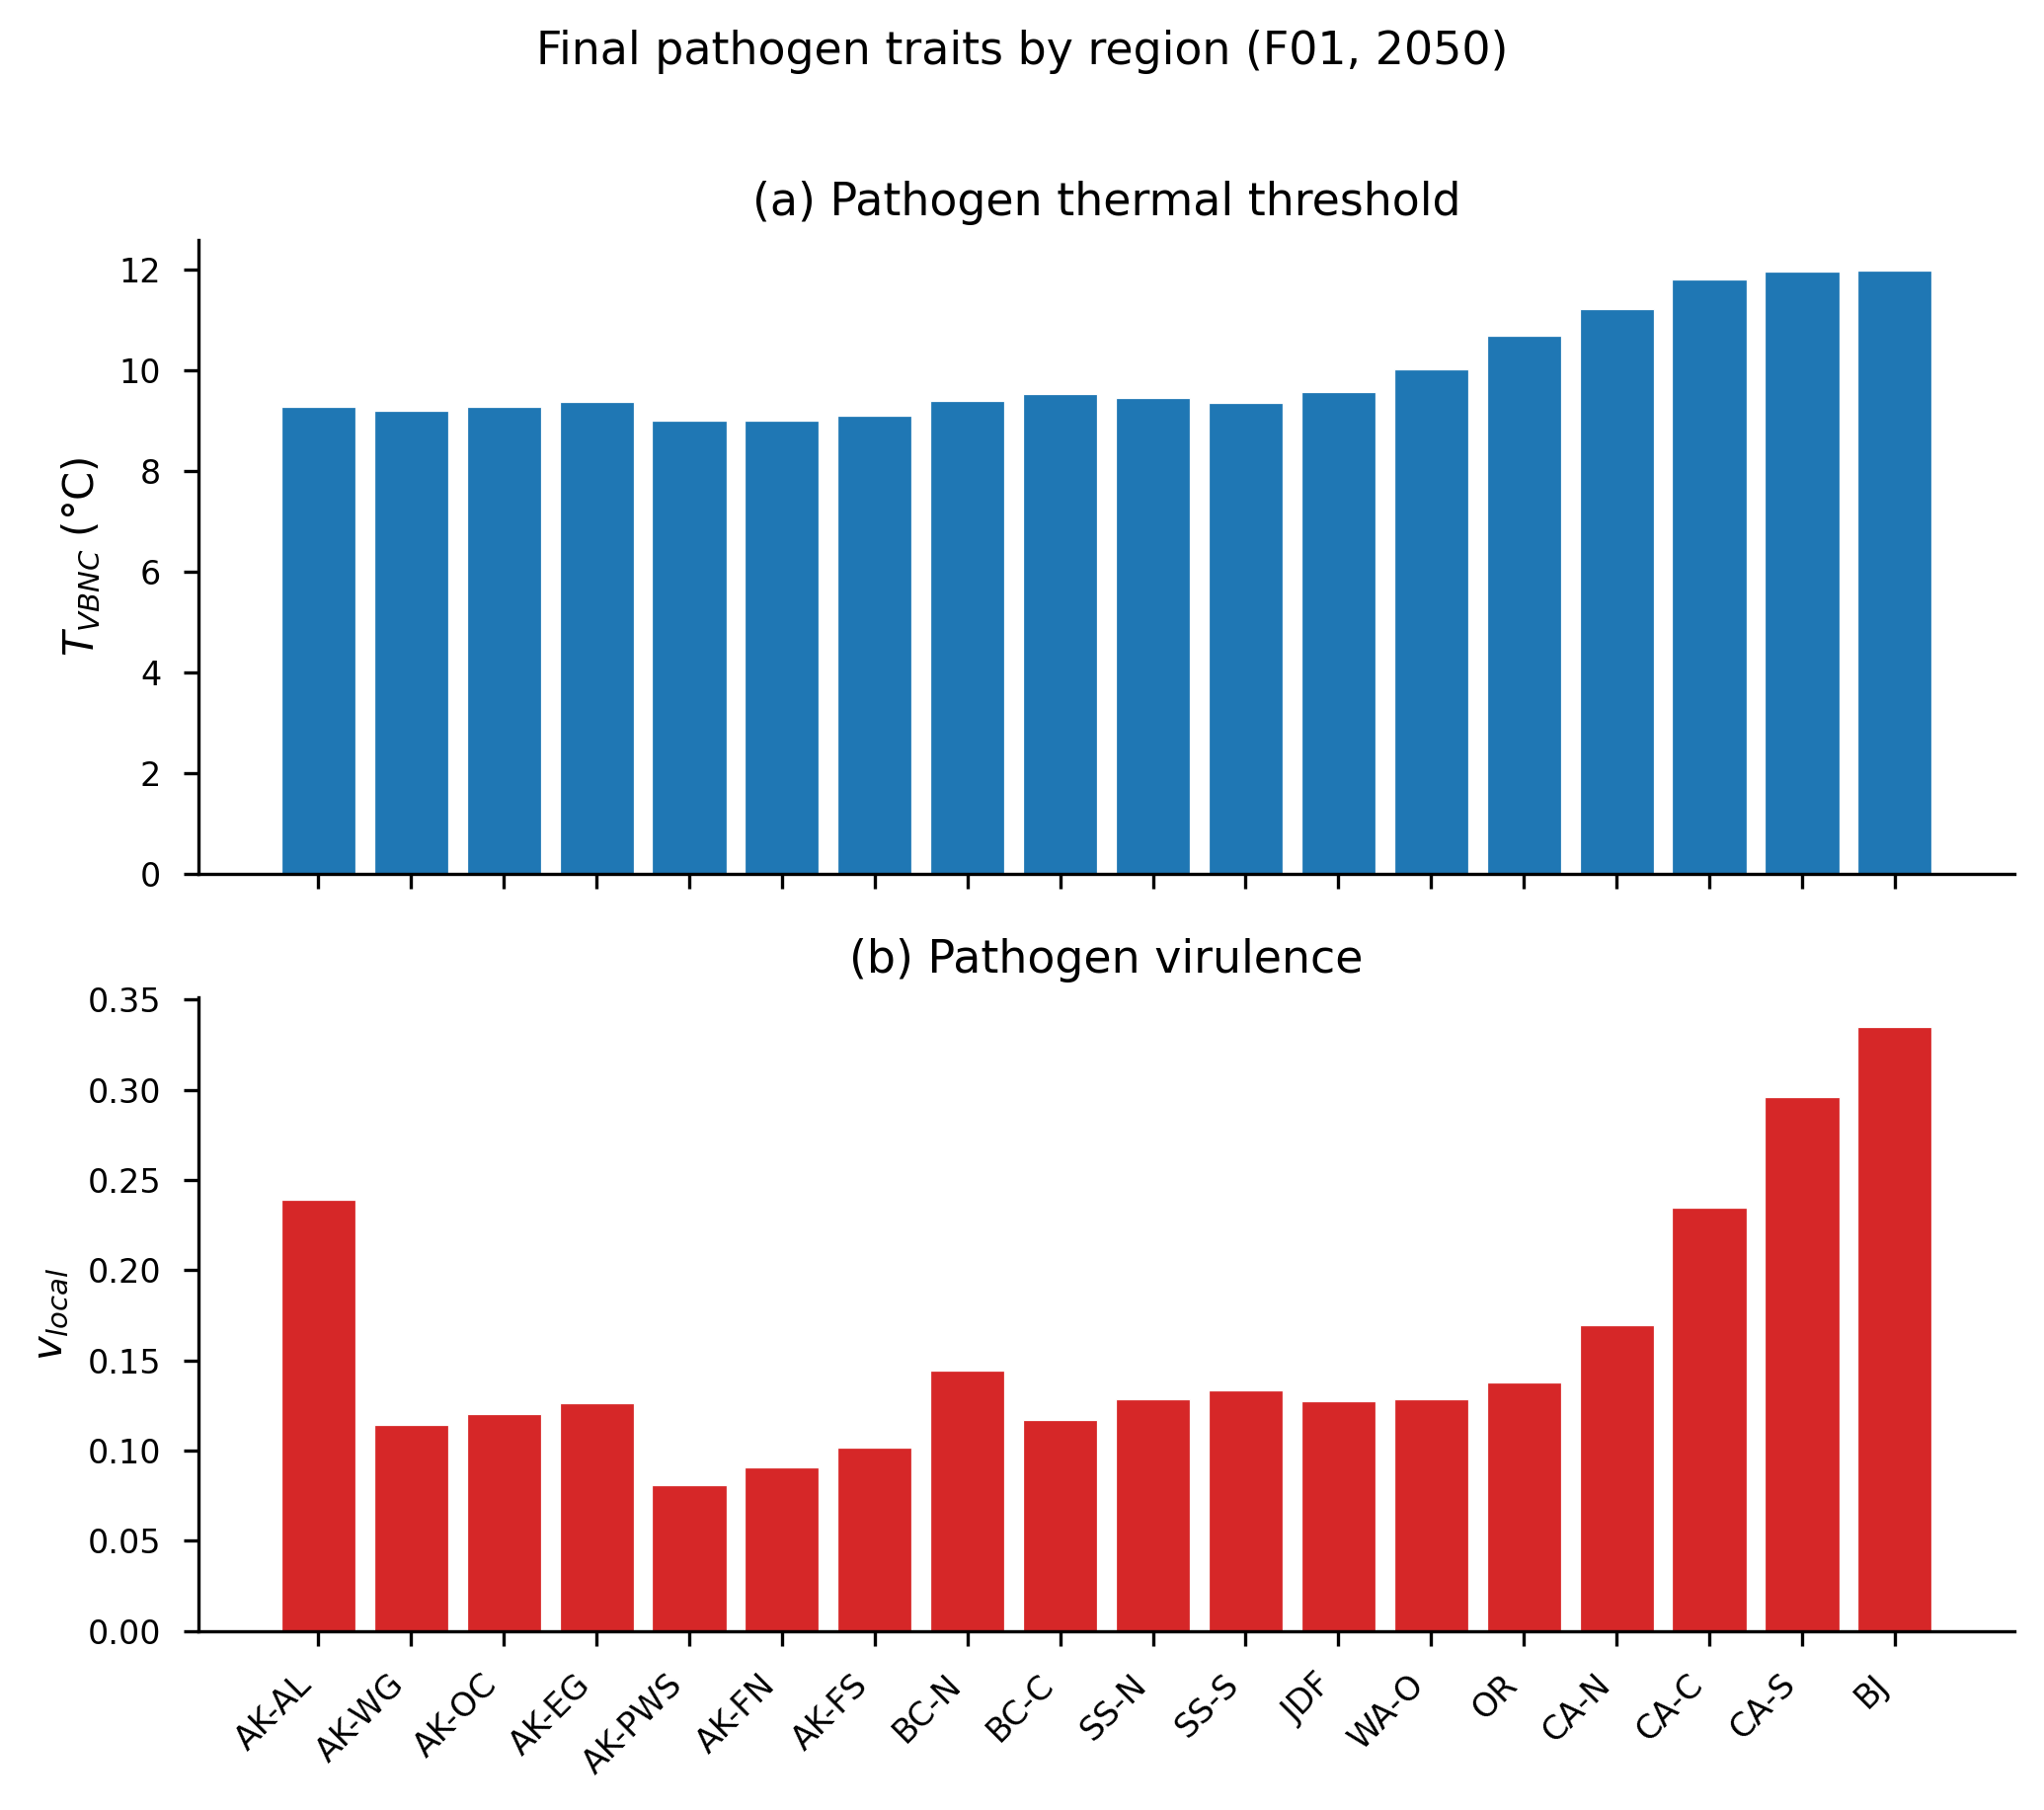
\includegraphics[width=0.75\textwidth]{figures/fig_pathogen_traits_final.png}
    \caption{Final (2050) pathogen community traits across all 18 regions under the baseline scenario (F01). \textbf{Top:} Thermal activation threshold ($T_{\text{vbnc}}$), showing how northern pathogen communities have evolved to activate at lower temperatures (reaching the 9\textdegree C biophysical floor throughout Alaska), while southern communities remain near the initial 12\textdegree C. \textbf{Bottom:} Local virulence ($v_{\text{local}}$), showing the latitudinal gradient predicted by virulence--transmission trade-off theory: high virulence in warm, dense southern waters (Baja: 0.34) and low virulence in cold, sparse northern waters (Alaska: 0.09).}
    \label{fig:pathogen_traits}
\end{figure>

At lower latitudes, $T_\mathrm{vbnc}$ settles at intermediate values
that reflect a balance between selection for broader thermal niches and
the diminishing marginal fitness return of further thermal adaptation
in already-warm environments:

\begin{itemize}
  \item BC-N: $T_\mathrm{vbnc} = 9.39$\textdegree C
  \item OR: $T_\mathrm{vbnc} = 10.70$\textdegree C
  \item CA-C: $T_\mathrm{vbnc} = 11.81$\textdegree C
  \item BJ: $T_\mathrm{vbnc} = 12.00$\textdegree C (upper bound,
    unchanged from initialization)
\end{itemize}

\noindent
The latitudinal gradient in $T_\mathrm{vbnc}$ is opposite to what
might na\"ively be expected.  In warm regions, the pathogen has no
``need'' to adapt its thermal niche because ambient temperatures
already exceed activation thresholds year-round; consequently,
$T_\mathrm{vbnc}$ remains near its initial value.  In cold regions,
even small reductions in $T_\mathrm{vbnc}$ substantially extend the
annual transmission window, creating strong selection for thermal
generalism.

The saturation of $T_\mathrm{vbnc}$ at 9.00\textdegree C throughout
Alaska by 2050 implies that pathogen thermal adaptation has effectively
reached its maximum extent in the north within the modeled range.
Further increases in pathogen pressure at high latitudes would require
either warming of SSTs above the adapted threshold for longer periods
or evolution of $T_\mathrm{vbnc}$ below the 9\textdegree C floor---a
possibility our model does not permit but that merits investigation in
future work.

\subsubsection{Virulence Gradient}

Local virulence ($v_\mathrm{local}$) evolves independently at each
site, driven by the interplay between within-host selection for
increased pathogen replication and the epidemiological cost of host
mortality.  By 2050, a pronounced latitudinal virulence gradient has
developed (Figure~\ref{fig:pathogen_traits}):

\begin{center}
\begin{tabular}{lc}
\toprule
\textbf{Region} & $v_\mathrm{local}$ (2050) \\
\midrule
AK-PWS & 0.081 \\
AK-FN  & 0.091 \\
BC-N   & 0.144 \\
OR     & 0.138 \\
CA-C   & 0.235 \\
BJ     & 0.335 \\
\bottomrule
\end{tabular}
\end{center}

\noindent
Virulence increases fourfold from Alaska (0.086) to Baja California
(0.343).  This gradient arises because southern populations sustain
chronic, dense pathogen populations year-round, favoring
aggressive strains that maximize short-term transmission.  In the
north, the annual interruption of transmission by winter cooling
selects against hyper-virulent strains that kill their hosts before the
next transmission season---a classic prediction of the
transmission--virulence trade-off hypothesis applied to a seasonally
structured environment \citep{alizon2009}.

The virulence gradient reinforces the north--south asymmetry already
created by climate: southern populations face not only longer pathogen
activity seasons but also intrinsically more virulent pathogen
populations, compounding the demographic disadvantage.

% ---------------------------------------------------------------------------
\subsection{The Pathogen Evolution Question}
\label{sec:pathogen_evo}

A central motivation of this study is to determine whether pathogen
evolution materially alters the long-term forecast for
\textit{P.~helianthoides}.  The factorial design permits direct
quantification of this effect through comparison of scenarios with
(F01) and without (F02) pathogen evolutionary capacity, and through the
intermediate case where only virulence evolution is disabled (F03).

\subsubsection{Aggregate Effect: Modest and Counterintuitive}

Coast-wide, disabling all pathogen evolution (F02) yields a modest
improvement: 5.9\% survival versus 5.4\% under F01, a difference of
$+$0.5 percentage points (Figure~\ref{fig:evo_comparison}).  This
result confirms the intuition that pathogen adaptation modestly
worsens host population outcomes, but the small magnitude is
surprising given the substantial trait changes documented in
Section~\ref{sec:evo_dynamics}.  Two features of the regional
breakdown are particularly unexpected.

\subsubsection{Where Disabling Evolution Hurts the Host}

Counterintuitively, removing pathogen evolution \textit{reduces}
recovery in Oregon ($-$4.8 percentage points: 17.6\% $\rightarrow$
12.8\%) and outer Washington ($-$3.7 points: 8.8\% $\rightarrow$
5.1\%).  These are among the most important recovery regions under the
baseline, and the loss is substantial.

The mechanism driving this paradox involves the interaction between
thermal adaptation and virulence evolution.  When pathogen evolution is
enabled (F01), the pathogen's VBNC threshold in the Pacific Northwest
declines from its initial value of 12.0\textdegree C toward
$\sim$10.6\textdegree C (Oregon), extending the pathogen's active
season by several weeks.  However, this same evolutionary process
simultaneously allows virulence to drift \textit{downward} from its
initial value toward a local optimum dictated by the
transmission--virulence trade-off.  In Oregon, evolved virulence
(0.136) is substantially below the pathogen's initial virulence
parameterization, meaning that the pathogen becomes less lethal per
transmission event even as it becomes more broadly active across
seasons.

When evolution is disabled (F02), the pathogen retains its initial
$T_\mathrm{vbnc}$ of 12.0\textdegree C, which in Oregon's thermal
regime restricts activity to a shorter summer window.  Crucially,
however, the pathogen also retains its initial virulence, which exceeds
the locally optimal value.  In the Pacific Northwest's thermal regime,
where winter cooling provides seasonal population recovery, the
combination of a shorter but more virulent active season (F02) proves
\textit{more damaging} than a longer but less virulent season (F01).
The elevated per-encounter lethality during the concentrated summer
peak overwhelms the benefit of a shorter overall transmission window.

This result has important biological implications: the net effect of
pathogen evolution on host populations is not uniformly negative.  In
thermally seasonal environments, the co-evolution of thermal niche and
virulence can produce a regime in which the pathogen becomes ``gentler
but more persistent''---a combination that, paradoxically, allows
greater host population recovery than the alternative of ``fierce but
brief'' epizootics.

\subsubsection{Where Disabling Evolution Helps the Host}

In most other regions, particularly at high latitudes, removing
pathogen evolution benefits the host.  The largest gains under F02
occur in:

\begin{itemize}
  \item BC-C: $+$4.2 points (3.3\% $\rightarrow$ 7.5\%)
  \item AK-AL: $+$3.7 points (0.4\% $\rightarrow$ 4.1\%)
  \item AK-WG: $+$2.0 points (2.5\% $\rightarrow$ 4.5\%)
  \item SS-S: $+$2.3 points (6.5\% $\rightarrow$ 8.8\%)
\end{itemize}

\noindent
In these cold-water regions, the dominant evolutionary axis is pathogen
thermal adaptation (downward movement of $T_\mathrm{vbnc}$), which
extends the pathogen's active season into previously safe shoulder
months.  Unlike in the Pacific Northwest, the virulence trade-off
provides little compensatory benefit here because the short active
season limits the number of transmission events over which reduced
virulence can accumulate a demographic advantage.  Consequently,
disabling evolution simply preserves the shorter pre-adaptation
activity window without offsetting virulence costs.

\subsubsection{Virulence Evolution Alone: A Minor Player}

Comparison of F01 (full evolution) with F03 (thermal adaptation on,
virulence off) isolates the specific contribution of virulence
evolution.  The effect is negligible: coast-wide survival changes from
5.4\% (F01) to 5.1\% (F03), a difference of only $-$0.3 percentage
points.  Regionally, the largest effects of disabling virulence
evolution alone are:

\begin{itemize}
  \item CA-N: $-$2.1 points (5.0\% $\rightarrow$ 2.9\%)
  \item OR: $-$2.3 points (17.6\% $\rightarrow$ 15.3\%)
  \item WA-O: $-$4.6 points (8.8\% $\rightarrow$ 4.2\%)
  \item AK-FN: $-$1.1 points (6.8\% $\rightarrow$ 5.7\%)
\end{itemize}

\noindent
These modest, mostly negative effects (i.e., disabling virulence
evolution slightly \textit{worsens} outcomes) are consistent with the
mechanism described above: virulence evolution tends to reduce
per-encounter lethality below initial values, providing a small net
benefit to host populations.  When this beneficial drift is prevented
(F03), outcomes are slightly worse.

Importantly, the contrast between the large effect of disabling
\textit{all} evolution (F02 vs.\ F01) and the small effect of
disabling virulence evolution alone (F03 vs.\ F01) implies that
\textbf{thermal adaptation is the dominant evolutionary axis} driving
the pathogen's impact on host populations.  Virulence evolution, while
biologically real and spatially structured, is a secondary modulator
whose effects are largely masked by the much larger influence of the
pathogen's expanding thermal niche.

\subsubsection{Synthesis: The Evolutionary Forecast}

The evolutionary analysis yields three key findings:

\begin{enumerate}
  \item \textbf{Pathogen evolution has a modest net negative effect
    on host populations} ($-$0.5\% coast-wide), but this aggregate
    conceals regionally divergent impacts that range from $+$4.8\% 
    (Oregon benefits from evolution) to $-$4.2\% (BC-C harmed by 
    evolution).
  \item \textbf{Thermal adaptation, not virulence evolution, is the
    primary driver.}  The pathogen's ability to expand its thermal
    niche and extend its active season is far more consequential than
    changes in per-encounter virulence.
  \item \textbf{The host's evolutionary response (increasing
    resistance) is substantial but insufficient.}  Even the most
    resistant surviving population (CA-C, $\bar{r} = 0.425$) still
    experiences more than half the disease mortality of na\"ive
    animals, and the populations most in need of evolutionary rescue
    are those least able to achieve it due to demographic collapse.
\end{enumerate}

\noindent
These results argue against a simple narrative of pathogen evolution as
uniformly detrimental and instead point to a complex, spatially
structured eco-evolutionary dynamic in which the net effect of
evolution depends critically on the local thermal regime, the seasonal
structure of transmission, and the interaction between thermal niche
expansion and virulence optimization.
